\section{Literature overview}
In this section, we cover the fundamental literature relative to the problem of the modeling of a flock of birds. We will follow an historical point of view, starting from C. Reynolds' pioneeristic "boids" model to Vicsek's active matter one and Couzin's "zonal" model. We then cover the importance of Cavagna et al.'s findings regarding the correlation function. In order for the discourse to flow conceptually, we must first cover the topic of emergence, perfectly crystallized by the famous essay "More is different" by P. W. Anderson \cite{more_is_different}.

\subsection{Many-body physics and emergence}
The reductionist hypothesis has, in the history of science, reigned sovereign as the basis of scientific inquiry; the possibility to reduce (hence the name) everything to a result of a number of fundamental laws is, self evidently, intrinsically captivating to the human spirit. Many-body physics is, to the reductionist worldview, a challenge in and of itself. The concept that governs this field is that of emergence, which is the manifestation of different, unpredictable symmetries from the ones that govern the fundamental parts of a many-body system.  A classic example is that of crystals: built according to perfectly homogeneous laws, the crystal unpredictably displays new symmetries. The general rule is, however, even in this case, that the system is less symmetrical than the underlying structure would suggest; as ordered as it
may be, a crystal is not perfectly homogeneous. More is different, in the words of P. W. Anderson; a concept that is perfectly explained in the closing of the eponymous article:

\begin{quote}
    \textit{ [...]I offer two examples from economics [...]. Marx said that quantitative differences become qualitative ones, but a dialogue in Paris in the 1920's sums it up even more clearly:}
    \begin{quote}
        \textit{\textsc{Fitzgerald}: The rich are different from us. \\
            \textsc{Hemingway}: Yes, they have more money. }\cite{more_is_different}
    \end{quote}
\end{quote}


\subsection{The flock of birds}
In light of the concepts covered in the last subsection, it should come as no surprise how large groups of animals have been studied as an example of emergence, considering how they behave. \\
The emergent property of a flock of birds that is first obvious to the eye is its capacity to move as one, and to react to predators and obstacles as such without dividing the flock. Since it is physically impossible for each and every bird to perceive each and every one of their flockmates, they must follow a set of simpler rules; the modeling of a flock of birds is inquiring into those rules. For most of the field's history, that meant reasonably guessing them and to evaluate, with a mixture of qualitative and quantitative methods, if the model behaved as a flock. This evaluation was intrinsically flawed, since it did not have real hard data to be tested against. This is where Cavagna's paper comes in handy. We will now explain three classical models for simulating a flock of birds, and then explain Cavagna's findings and how they can be used to test the aformentioned models.
\subsubsection{Reynolds' model: the "boids"}
\label{subsec:boids}
The first model, historically, is the one named "boids", by Craig Reynolds. He set out to animate bird-oid objects (hence the name "boids") which moved based on a simple set of three rules:
\begin{figure}
    \centering
    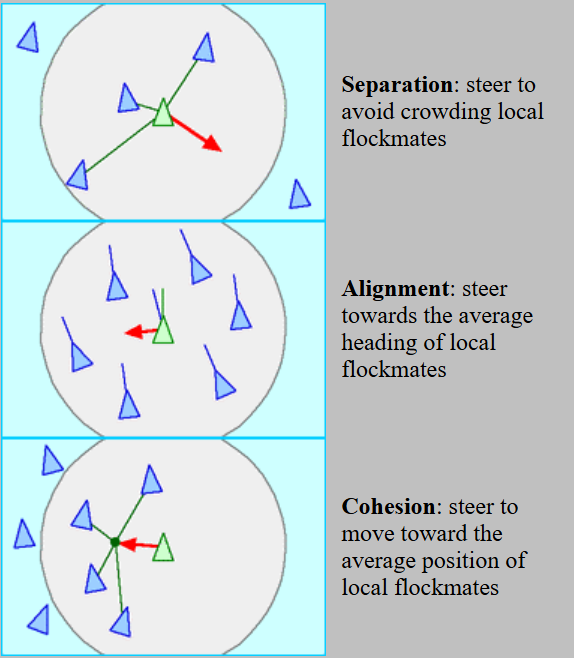
\includegraphics[width=0.8\linewidth]{pictures/sec_2/boids.png}
    \caption{Pictorial representation of the boids' rules from Reynolds' personal site. \cite{reynolds_site}}
    \label{fig:boids}
\end{figure}
\begin{itemize}
    \item \textbf{Cohesion:} the boids tend to be attracted to the centroid of nearby flockmates;
    \item \textbf{Alignment:} the boids tend to align their direction with that of nearby flockmates;
    \item \textbf{Separation:} the boids tend to be repelled by nearby flockmates;
\end{itemize}
It should be noted that the distance that defines "nearby" is the same for all three of the forces, as suggested by \autoref{fig:boids}. \\ Reynolds also used some more rules in order for the model to behave more realistically \cite{boids}, some of which were later refined in a more recent paper \cite{reynolds_1999}:
\begin{itemize}
    \item \textbf{Maximum speed:} in order to ensure that no boid gets too fast too quick and escapes the flock, the speed gets capped;
    \item \textbf{Minimum speed:} in order to ensure that the flock does not become stagnant, no boid can get slower than an arbitrary threshold;
    \item \textbf{Limited acceleration:} to simulate more realistic behaviour, boids can accelerate only for a limited amount;
    \item \textbf{Limited field of view:} to simulate more realistic behaviour, every boid has a limited peripheral perception, namely it does not react to the boids behind him;
\end{itemize}
The limited steering actually has another effect, considering the way Reynolds explains the implementation of the model; namely, he implements each rule's effect on an accumulator, and gives an order to them, specifically separation, alignment and cohesion. What this means, operatively, is that if the sum of two or three forces exceeds the magnitude given by the limited steering, only the last one or two applied will be rescaled.  Also, if either alignment or separation exceed the maximum steering and so saturate the accumulator, cohesion does not operate on the boid. In the latter case, alignment does not operate either.\\
Considering that he is an Academy award winning computer graphic scientist, specialized in the simulation of natural phenomena for the entertainment industry \cite{reynolds}, his model only aims at a qualitative representation of a flock: that means that the only test he truly cares about is the eye test, as stated in the original '87 paper \cite{boids}. This is a key detail for our dissertation.
\subsubsection{Vicsek's model: self propelled particles}
\begin{figure}[h]
    \centering
    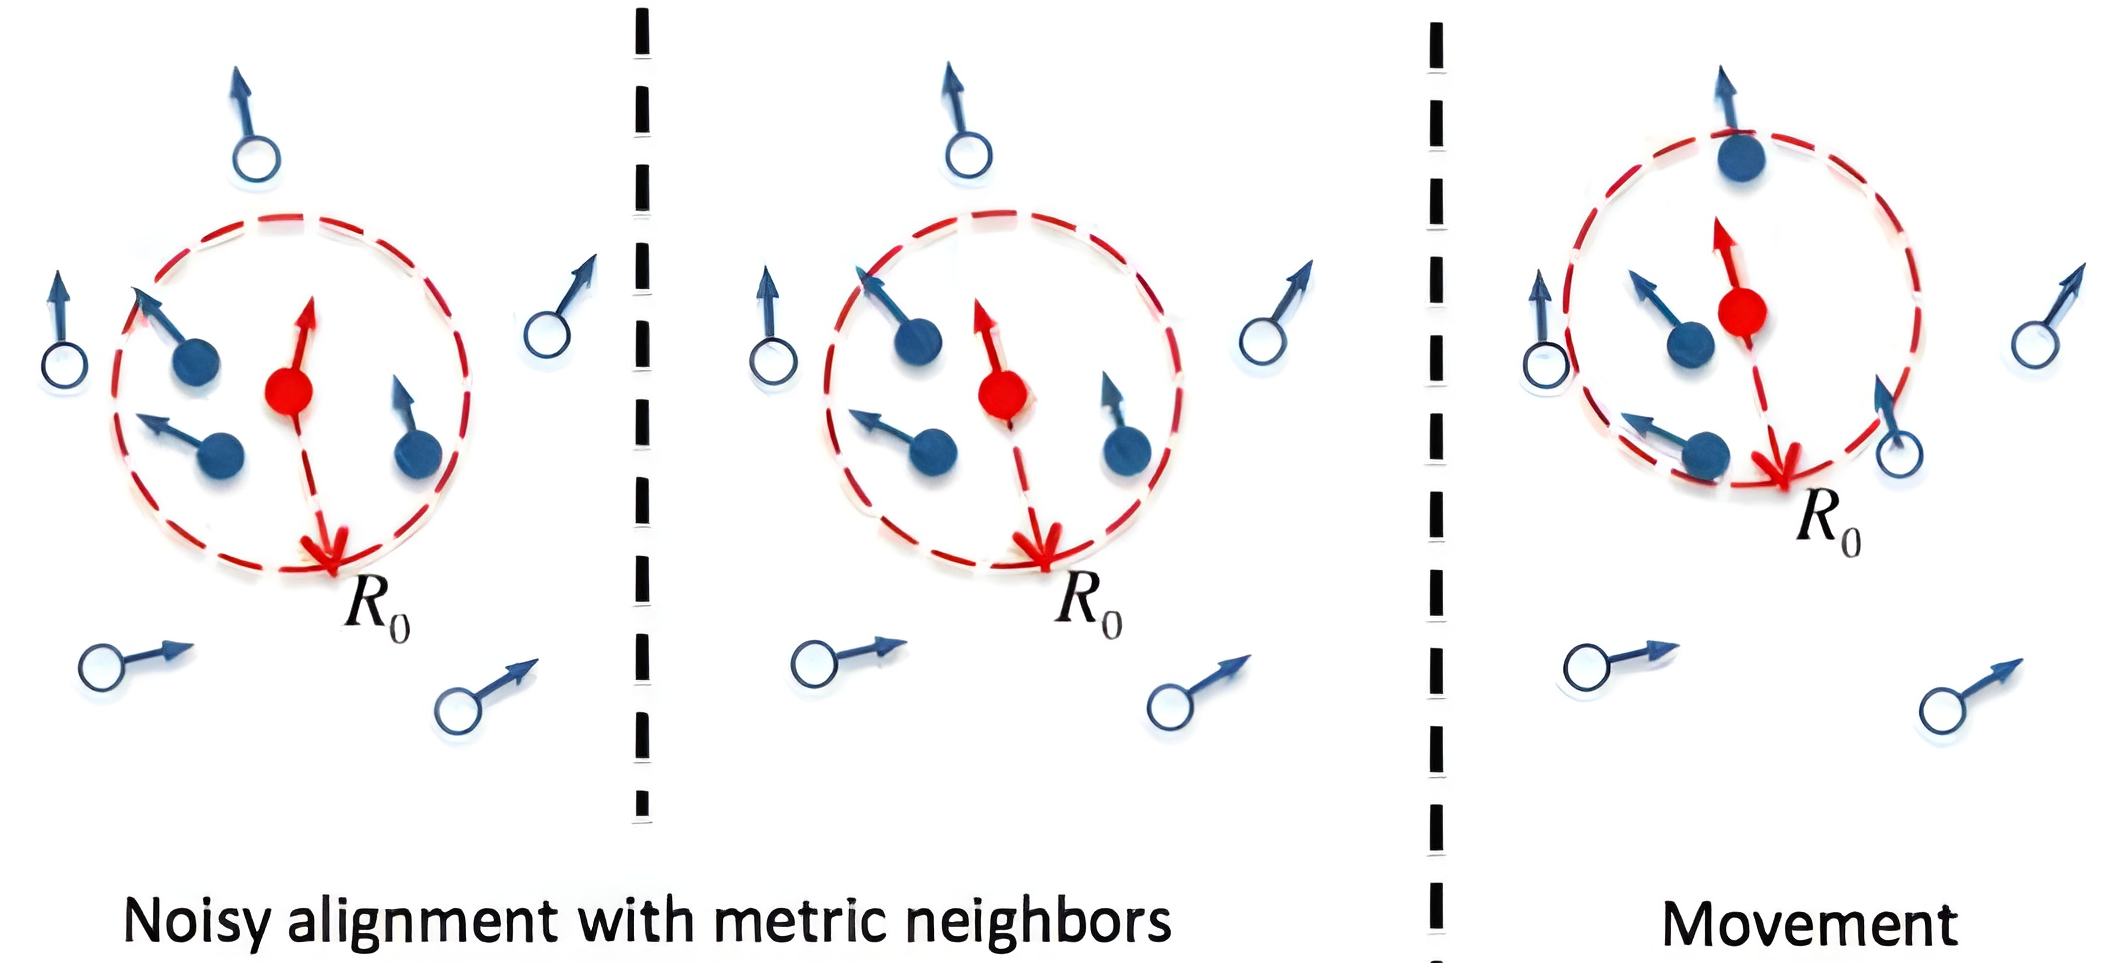
\includegraphics[width=0.99\linewidth]{pictures/sec_2/vicsek.png}
    \caption{Representation of the behaviour of a particle in Vicsek's model. \cite{vicsek_manual}}
    \label{fig:vicsek}
\end{figure}
A simplification of Reynolds' model, Vicsek's was created as means of studying active matter, as the name of the original paper suggests. Vicsek's interest lays in phase transitions in systems of self propelled particles. Consequently, his model tried to emulate this kind of system with a toroidal space. \cite{vicsek_manual} \\
Derivatively from the alignment constraint in the "boids" model, Vicsek's is based on one simple rule; from the words of the man himself:

\begin{quote}
    \textit{The only rule of the model is: at each time step a given particle driven with a constant absolute velocity assumes the average direction of motion of the particles in its
        neighbourhood of radius $r$ with some random perturbation added, as shown in \autoref{fig:vicsek}.} \cite{vicsek}
\end{quote}
The aforementioned rule, when calling the random noise $\Delta\theta$, reads as:
\begin{equation}
    \label{eq:vicsek}
    \begin{split}
        \theta(t + 1)             & = \langle\theta(t)\rangle_r + \Delta\theta                      \\
        \langle\theta(t)\rangle_r & = \frac{1}{N_{neighbours}} \sum_{|x_j - x_i| \le r} \theta_j(t)
    \end{split}
\end{equation}
His model does have one additional constraint, namely uniform speed \cite{vicsek_manual}; it should also be noted that since technically it is not trying to emulate birds but particles, all of the rules that apply to other models to simulate realistic behaviour (i. e. limited FOV, limited steering) do not make sense for Vicsek's model.
By simulating a system that obeyed \autoref{eq:vicsek}, Vicsek was able to observe phase transitions and flocking; in other words, the system exhibited order from a not ordered starting point \cite{vicsek}; as much as the model is not based on the behaviour of flocks of birds, it does nontheless exhibit similar collective patterns as them, as Vicsek claims(although that was later attributed to the use of  a toroidal space \cite{chate}), which is why we decided to include it in this work. \\
Since Vicsek is a physicist, he does perform quantitative analysis, but considering that the scope of his work is different than ours, they are not relevant for our own dissertation.
\subsubsection{Couzin's model: the "zonal" algorithm}
\begin{figure}[h]
    \centering
    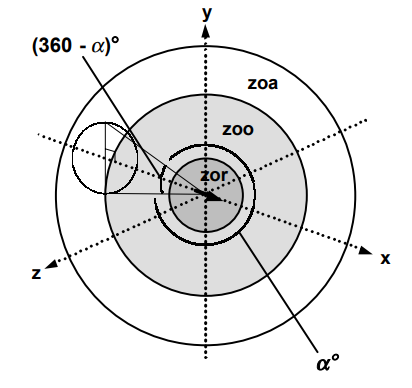
\includegraphics[width=0.85\linewidth]{pictures/sec_2/couzin.png}
    \caption{Representation of an individual in the model centered in the origin. \textit{zoo} stands for zone of orientation, \textit{zoa} for zone of attraction and \textit{zor} for zone of repulsion.}
    \label{fig:couzin}
\end{figure}
An advancement more from Reynolds' than from Vicsek's model is the one by Ian D. Couzin, often referred to as the "zonal" model for reasons that will be self evident in a moment. \\
Couzin, like Reynolds, asserts that every bird should be dominated by three forces: attraction, orientation and repulsion, which respectively correspond to cohesion, alignment and separation defined for the "boids" model in \autoref{subsec:boids}. The similarity to Vicsek's model, instead, lies in the fact that the speed is fixed.
Couzin defines the forces' effects algebraically, more specifically every interaction should determine the direction in the following time step as follows:
\begin{equation}
    \label{eq:couzin_r}
    \mathbf{d}_r(t + \tau) = -\sum_{j \neq i}^{n_r} \frac{\mathbf{r}_{ij}(t)}{|\mathbf{r}_{ij}(t)|}
\end{equation}
\begin{equation}
    \label{eq:couzin_o}
    \mathbf{d}_o(t + \tau) = \sum_{j=1}^{n_o} \frac{\mathbf{v}_j(t)}{|\mathbf{v}_j(t)|}
\end{equation}
\begin{equation}
    \label{eq:couzin_a}
    \mathbf{d}_a(t + \tau) = \sum_{j \neq i}^{n_a} \frac{\mathbf{r}_{ij}(t)}{|\mathbf{r}_{ij}(t)|}
\end{equation}
The key difference from Reynolds' model lies in when the forces act. Couzin defines three zones, one for every interaction. The zone of repulsion is the one with the smaller radius, and as such is a spherical sector, in order to account for the bird's limited FOV. The zones of orientation and attraction are instead sectors of spherical shells (again to emulate the limited FOV), and the zone of attraction is the largest one, as shown in \autoref{fig:couzin}. When a bird has any neighbours in the zone of repulsion, \autoref{eq:couzin_r} applies for the whole set of $n_r$ neighbours. Repulsion takes precedence: if and only if $n_r=0$ the other forces may apply. In particular, if there is a number of neighbours only in one of the other zone, only the corresponding force applies, if there are some in both, $\mathbf{d}(t+\tau)=\frac{\mathbf{d}_o(t+\tau)+\mathbf{d}_a(t+\tau)}{2}$ \cite{couzin}.\\
Couzin, akin to Vicsek, is a scientist (a biologist to be precise) and as such he performs some qualitative analysis of his model. We will not cover them extensively because the analysis in Cavagna's group's work is more thorough.

\subsection{Cavagna's findings: the first experimental dataset and the first emergent property}

In 2008, it was found that the flocking birds' criteria for interaction are not metric, but topological: specifically, birds interact with their closest six or seven neighbours \cite{bellerini}. Cavagna and his group, by using a dataset of which the specifics can be read at \cite{cavagna2008starflag1} \cite{cavagna2008starflag2}, wanted to refine that claim. Specifically, they wanted to understand the scale of the system's correlation. Cavagna asserts that the main emergent behaviour in a flock is not its order, but its collective reaction, be it to predators or obstacles; his hypothesis is that it cannot possibly be a result of a movement that is correlated with just the six or seven closest neighbours' one \cite{cavagna_2010}. A didactic example, in this sense, is that of the "telephone" game, in which one says something and their neighbour communicates said thing to their own neighbour, and so on; if every one communicates effectively, although each player only directly communicates with their neighbours, the final message is correlated with the initial one. The key takaway from the telephone game example is that interaction range and correlation range could be different, even dramatically so.\\
\begin{figure}[h]
    \centering
    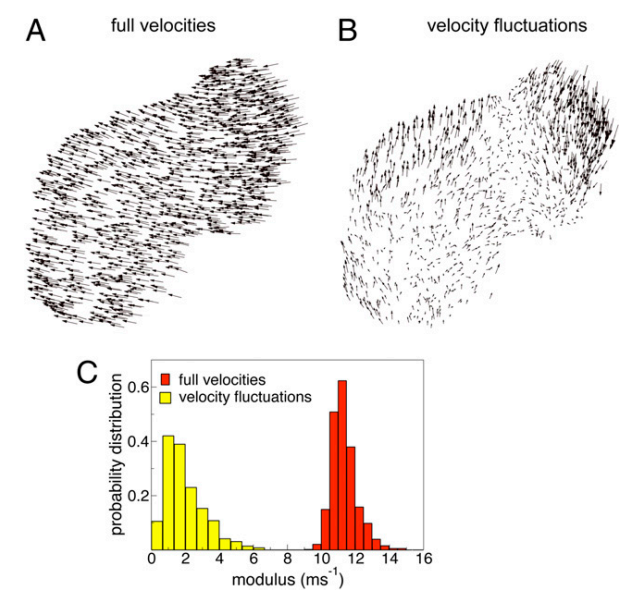
\includegraphics[width=0.85\linewidth]{pictures/sec_2/cavagna_vel_fluc.png}
    \caption{2d projections of an arbitrary flock's velocity and velocity fluctuations, combined with their distribution.}
    \label{fig:cavagna_vel_fluc}
\end{figure}
Cavagna, differently from his predecessors, has empirical data: that means that his analysis is rooted in (empirical) reality, and he can consequently prove (or disprove) his hypothesis. By analyzing the data, his group observed how the velocity fluctuations tended to be grouped in two regions of the flock, as seen in \autoref{fig:cavagna_vel_fluc}. In order to crystallize this observation mathematically, his group defined the correlation function $C(r)$ as:
\begin{equation}
    \label{eq:correlation_function}
    C(r) = \frac{1}{c_0} \frac{\sum_{ij} \vec{u}_i \cdot \vec{u}_j \, \delta(r - r_{ij})}{\sum_{ij} \delta(r - r_{ij})}
\end{equation}
where $\vec{u}_i = \vec{v}_i - \frac{1}{N} \sum_{k=1}^N \vec{v}_k,$ is the fluctuation around the mean flock’s velocity for for each bird $i$, $\delta(r - r_{ij})$ is a smoothed Dirac $\delta$-function selecting pairs of birds at mutual distance $r$; $\vec{u}_i \cdot \vec{u}_j = u_i^x u_j^x + u_i^y u_j^y + u_i^z u_j^z$ and $c_0$ is a normalization factor (of dimension $\text{m}^2 \cdot \text{s}^{-2}$) such that $C(r = 0) = 1$ \cite{cavagna_2010}. \\
By looking at the same image, one can see how the velocities, differently from their fluctuations, are well aligned. To quantify this global ordering, they inquired about its polarization, which is defined as such:
\begin{equation}
    \Phi=\left|\left|\frac{1}{N}\sum_{i=1}^N\frac{\vec{v_i}}{||\vec{v_i}||}\right|\right|
\end{equation}
In the paper, they obtain an average value of $\Phi=0.96\pm0.03$\cite{cavagna_2010}. \\
The correlation function, as defined in \autoref{eq:correlation_function}, should span between 1 and -1, and positive values represent positive correlation while negative ones represent anti-correlation. A single-signed section should represent a subgroup of the flock that reacts in the same way. \\
\begin{figure}[h]
    \centering
    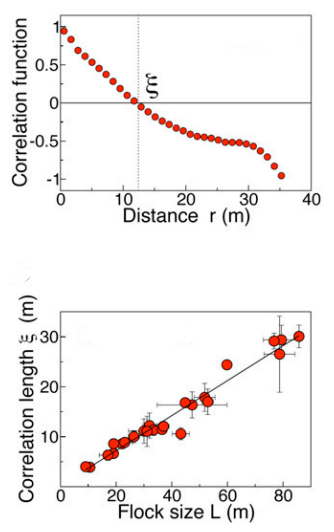
\includegraphics[width=0.75\linewidth]{pictures/sec_2/cavagna_correlation_function.png}
    \caption{Plotting of the correlation function of a flock, and of the intercept $\xi$ of many flocks' correlation function against their size.}
    \label{fig:cavagna_correlation_function}
\end{figure}
By analyzing \autoref{fig:cavagna_correlation_function},  we can finally infer what Cavagna's paper asserts with greater theoretical rigour: the flock's correlations are scale-free, and all flocks behave the same, as $\xi$, the correlation length, grows linearly with their size. The non-trivial part is that the correlation function $C(r)$ only has two single-signed sections, which can heuristically explain how the interactions are scale-free: the whole flock reacts to each and every bird's movement either in a positive way or a negative one; in other words, there are only two domains of reaction: either compliant or opposite \cite{cavagna_2010}. \\
The claim is refined, in the a later paper, by employing the methods of statistical mechanics. With the idea in mind to find a statistical model for the flock, they used the maximum entropy (MaxEnt)principle, which states that the most assumption-less model (not necessarily the most correct one) is the one that maximises the entropy of the system, given some constraints. In this case, the MaxEnt distribution is:
\begin{equation}
    P(\{\vec{s}_i\}) = \frac{1}{Z(\{J_{ij}\})} \exp \left[ \frac{1}{2} \sum_{i=1}^{N} \sum_{j=1}^{N} J_{ij} \vec{s}_i \cdot \vec{s}_j \right]
    \label{eq:MaxEnt}
\end{equation}
Where $Z(\{J_{ij}\})$ is the proper normalization factor, and $J_{ij}$ is calculated in order for the predicted correlation function to be the same as the empirical one; this is one of our constraint. The most logical simplification of \autoref{eq:MaxEnt} is the one in which every boid interacts with a limited number of neighbours $n_c$ with the same intensity (or weight) $J$:
\begin{equation}
    P(\{\vec{s}_i\}) = \frac{1}{Z(J, n_c)} \exp \left[ \frac{J}{2} \sum_{i=1}^{N} \sum_{j \in n_c^i} \vec{s}_i \cdot \vec{s}_j \right]
    \label{eq:simpMaxEnt}
\end{equation}
where $j\in n_c^i$ means that bird j belongs to the first $n_c$ nearest neighbors of i. As it turns out, this model is incredibly predictive, and confirms once again that the interactions are scale-free and most importantly topological, as proved by the fact that the $n_c$ that maximizes the $P(\{\vec{s}_i\})$ in \autoref{eq:simpMaxEnt} is steady in regards to the size of the analyzed flock. \cite{cavagna_2012} \\
The gist of the whole analysis by Cavagna's group is that the  interactions between birds in a flock are indeed topological and not metric, but while finding that out, they discovered the emergent properties we will analyze for other, less recent models.

